\documentclass[11pt,a4paper]{article}

% Encoding and languages
\usepackage[utf8]{inputenc}
\usepackage[T1]{fontenc}
\usepackage[english]{babel}

% Mathematics and symbols
\usepackage{amsmath}
\usepackage{graphicx}
\usepackage{caption}
\usepackage{subcaption}
\usepackage{geometry}
\usepackage{newpxtext}
\usepackage{newpxmath}
\usepackage{microtype}
\usepackage{csquotes}
\usepackage{hyperref}
\usepackage{cleveref}
\usepackage{listings}
\usepackage{tcolorbox}
\usepackage{float}
\usepackage{placeins}

% Margin configuration
\geometry{left=2.5cm,right=2.5cm,top=2.5cm,bottom=2.5cm}

% Link configuration
\hypersetup{
    colorlinks=true,
    linkcolor=blue,
    filecolor=magenta,      
    urlcolor=cyan,
    citecolor=red,
    pdftitle={SiraEdge - Portfolio Optimization Module},
    pdfauthor={Ismail Moudden},
    pdfsubject={Quantitative Portfolio Optimization},
    pdfkeywords={finance, optimization, portfolio, machine learning, risk parity}
}

% Listings configuration
\lstset{
    basicstyle=\ttfamily\small,
    breaklines=true,
    frame=single,
    numbers=left,
    numberstyle=\tiny,
    showstringspaces=false,
    tabsize=2,
    captionpos=b
}

% tcolorbox configuration
\tcbuselibrary{skins}
\tcbset{
    enhanced,
    colback=blue!5,
    colframe=blue!75!black,
    fonttitle=\bfseries,
    boxrule=0.5pt
}

% Macro for handling missing figures
\newcommand{\maybeincludegraphics}[2][]{%
    \IfFileExists{#2}{\includegraphics[#1]{#2}}{\fbox{Missing figure: #2}}
}

% Figure path
\graphicspath{{../../figures/}{../../}}

\begin{document}

\title{\textbf{SiraEdge - Portfolio Optimization Module}\\[0.9em]
\large{Research and Implementation of Quantitative Models}}

\author{Ismail Moudden\\[0.6em]
\textit{SiraEdge — Portfolio Optimization Module}}

\date{\today}

\begin{titlepage}
\thispagestyle{empty}
\maketitle
\vspace{2em}

\begin{abstract}
This report presents the portfolio optimization module developed for the SiraEdge platform, an innovative solution aimed at democratizing access to professional asset management tools. We detail the implementation, comparative analysis, and validation of seven optimization models: Markowitz, Risk Parity, Monte Carlo, Black-Litterman, Machine Learning, Hybrid, and Custom Metrics. The study includes a robust walk-forward analysis and performance evaluation on real data (2020-2023). All source codes, figures, and results are available in the associated GitHub repository.
\medskip\par\noindent\textit{Scope.} This document is a \textbf{technical and educational report} showcasing the results of research and implementations; it constitutes \emph{neither an allocation recommendation}, \emph{nor a promise of future performance}.
\end{abstract}

\vfill
\end{titlepage}

\section*{SiraEdge Context and Vision}

\subsection*{Our Mission}
SiraEdge was born from a simple yet ambitious vision: \textbf{to democratize access to professional portfolio management tools}. Our mission is to make finance accessible to everyone by combining mathematical rigor with intuitive user experience.

\subsection*{The SiraEdge Platform}
SiraEdge is an interactive platform developed for learning to invest and simulating portfolios. It integrates several modules:
\begin{itemize}
    \item \textbf{Portfolio Simulation}: Testing strategies without risk
    \item \textbf{Optimization Module}: This report presents this module
    \item \textbf{Interactive Learning}: Tutorials and educational resources
    \item \textbf{Performance Analysis}: Advanced metrics and visualizations
\end{itemize}

\subsection*{Context of this Optimization Module}
This document presents \textbf{the concrete result of R\&D work and implementation} of the optimization models integrated into SiraEdge. The objective is \textbf{to showcase the fruits of research} (codes, figures, protocols) and provide a reproducible foundation. This is not an investment recommendation, but a \emph{technical and educational report}.

\begin{itemize}
    \item Making available ready-to-use scripts for generating figures
    \item Comparing models on a consistent test universe (2020--2023)
    \item Explaining risk/return trade-offs and practical limitations
    \item Documenting hyperparameter choices and backtesting protocols
\end{itemize}

\subsection*{Positioning in the SiraEdge AI Assistant}
In SiraEdge, the AI assistant is \textbf{a chatbot for help and analysis}: it answers user questions, explains figures, and \textbf{analyzes strategies} using available metrics (Sharpe, Sortino, Calmar, stability, turnover). It can compare models and interpret results, but \textbf{it does not provide personalized investment recommendations}. The graphs and tables in this report constitute its technical knowledge base.

\subsection*{Report scope — what it is / what it is not}
\textbf{What it is}
\begin{itemize}
  \item A report on R\&D and integration of models (Markowitz, Risk Parity, BL, ML, Hybrid, etc.)
  \item Support for the AI assistant to illustrate concepts and results
  \item A reproducible backtesting protocol with standardized metrics
\end{itemize}
\textbf{What it is not}
\begin{itemize}
  \item A turnkey trading strategy or personalized recommendation
  \item A marketing study; the numbers serve \emph{learning} and comparison
  \item A commitment to future performance; the universe and period are for demonstration
\end{itemize}

\subsection*{Backtesting and statistics in SiraEdge}
The optimization engine is connected to SiraEdge's \textbf{backtesting module}. The scripts produce return series and metric tables (Sharpe, Sortino, Calmar, weight stability, turnover) that feed the \texttt{Statistics} and \texttt{Simulation} pages. The results are presented \textbf{for comparative and educational purposes} and may differ from future performance; the numbers depend on the period (2020--2023), the chosen universe, and assumptions (costs, constraints).

\subsection*{Educational Approach}
Our approach combines:
\begin{itemize}
    \item \textbf{Scientific Rigor}: Faithful implementation of academic models
    \item \textbf{Accessibility}: Clear explanations and concrete examples
    \item \textbf{Reproducibility}: Complete source code and detailed documentation
\end{itemize}

\subsection*{GitHub Repository}
All source codes, figure generation scripts, and resources for this project are available in the GitHub repository:
\begin{center}
\textbf{\url{https://github.com/SiraEdge/portfolio-optimization}}
\end{center}

\textbf{Repository Structure:}
\begin{itemize}
    \item \texttt{src/}: Python implementation of all models
    \item \texttt{figures/}: Generated graphs and visualizations
    \item \texttt{rapport/}: LaTeX sources for this report
    \item \texttt{README.md}: Installation and usage instructions
    \item \texttt{requirements.txt}: Python dependencies
\end{itemize}

\textbf{Important note:} This report references specific code files. For complete understanding and the ability to reproduce results, it is essential to consult the associated GitHub repository.

\newpage

\tableofcontents

\newpage

\section{Introduction}
This report presents, in an educational and reproducible framework, several portfolio optimization approaches: classical models, machine learning-driven methods, hybrid variants, and optimization through custom metrics. The figures are generated by Python scripts (in the \texttt{src/} folder) and referenced here.

\begin{tcolorbox}[title=Research context and objectives]
This document presents a portfolio allocation framework compliant with academic standards: formal model exposition, explicit assumptions, experimental protocol, hyperparameters, results, and critical analysis. The ambition is to produce a \emph{reproducible} artifact (scripts, figures, dependencies) and \emph{interpretable} (justification of choices and limitations).
\end{tcolorbox}

\section{Concepts and Terminology}

\subsection{Fundamental finance concepts}

\textbf{Portfolio:} This is simply a collection of assets (stocks, bonds, etc.) in which you place your money. Think of it as a basket with different fruits - each fruit represents an asset, and the quantity of each fruit represents the weight of that asset in the portfolio.

\textbf{Return:} This is the gain or loss as a percentage over a period. If you buy a stock at \$100 and it's worth \$110 a year later, the return is 10\%. In finance, we often use \emph{logarithmic returns} because they add up better over time.

\textbf{Volatility:} This is a measure of the instability of an asset's price. The more volatile an asset, the more its price can rise or fall rapidly. It's like a car driving fast - it can go far but also skid more easily.

\textbf{Correlation:} Measures how much two assets move together. If two stocks rise and fall at the same time, they are positively correlated. If one rises when the other falls, they are negatively correlated. A correlation of 0 means they move independently.

\subsection{Analysis and testing tools}

\textbf{Backtest:} This is like "replaying history" with an investment strategy. We take past data and simulate what would have happened if we had applied our strategy at that time. It's useful for testing ideas without risking real money, but beware: the past doesn't guarantee the future!

\textbf{Walk-forward:} A more sophisticated technique than simple backtesting. Instead of testing on the entire history, we test on sliding windows (for example, 252 days = 1 trading year). This better simulates reality where we only know the past to make decisions.

\textbf{Rebalancing:} The action of modifying asset weights in the portfolio to return to the target allocation. For example, if the goal is 50\% stocks + 50\% bonds, and after a year stocks are worth 60\% of the portfolio, we sell stocks to buy bonds.

\subsection{Investment styles}

\textbf{Defensive:} A strategy that prioritizes stability and capital protection over maximum performance. We accept lower returns to avoid large losses. It's like driving carefully on a slippery road.

\textbf{Low turnover:} A strategy that limits frequent changes in the portfolio. The less we move, the less we pay in transaction costs. It's like a gardener who lets his plants grow rather than constantly moving them.

\textbf{Core-satellite:} An approach that combines two strategies: a stable "core" that represents the majority of the portfolio, and a more dynamic part (satellite) to try to improve performance. It's like having a solid house (core) and an ornamental garden (satellite).

\subsection{Performance metrics}

\textbf{Sharpe Ratio:} Measures the efficiency of an investment by comparing excess return (relative to the risk-free rate) to volatility. The higher it is, the better. It's like measuring how many kilometers you get per liter of gas - you want maximum return for minimum risk.

\textbf{Sortino Ratio:} Similar to Sharpe, but only penalizes "negative" volatility (losses). This is more logical because we worry more about losses than gains.

\textbf{Calmar Ratio:} Compares annualized return to maximum drawdown (largest loss over a period). The higher it is, the faster the portfolio recovers from its losses.

\textbf{Maximum Drawdown (MDD):} Largest loss as a percentage from a peak. If your portfolio was worth \$100, then \$80, then \$90, the MDD is 20\% (from \$100 to \$80).

\textbf{Weight stability:} Measures how much the portfolio allocation remains stable over time. Weights that change little mean fewer transaction costs and a more predictable strategy.

\textbf{Turnover:} Measures trading activity. A turnover of 100\% means we traded the equivalent of 100\% of the portfolio value over the period. The higher it is, the more transaction costs impact performance.

\subsection{Costs and constraints}

\textbf{Transaction costs:} Costs paid on each buy or sell (broker commissions, spreads, etc.). Generally expressed in "basis points" (bps): 1 bps = 0.01\%. Costs of 5 bps mean we pay 0.05\% on each transaction.

\textbf{Weight constraints:} Limits imposed on each asset's share. For example, "no more than 20\% in a single stock" or "at least 10\% in cash". These constraints often reflect risk management rules or regulatory preferences.

\section{Data and Preprocessing}
\subsection{Assets and period}
We use daily prices (2020--2023) for the following assets: ETFs \texttt{SPY}, \texttt{QQQ}, \texttt{IWM}, \texttt{EFA}; commodities \texttt{GLD}, \texttt{SLV}, \texttt{USO}, \texttt{DBA}. Data is downloaded via \texttt{yfinance}.

\subsection{Returns and indicators}
The \textbf{logarithmic returns} of a price \(P_t\) are defined by \(r_t = \ln(P_t/P_{t-1})\). They add up over time and approximate simple returns well for small variations.
\textbf{Momentum} here refers to a cumulative short-term variation (e.g., 20 days), \textbf{rolling volatility} a local dispersion measure, and \textbf{RSI} (Relative Strength Index) a bounded oscillator \([0,100]\) capturing the speed of rises/falls. Figure \ref{fig:corr_external} shows the correlation between assets.

\begin{figure}[h]
  \centering
  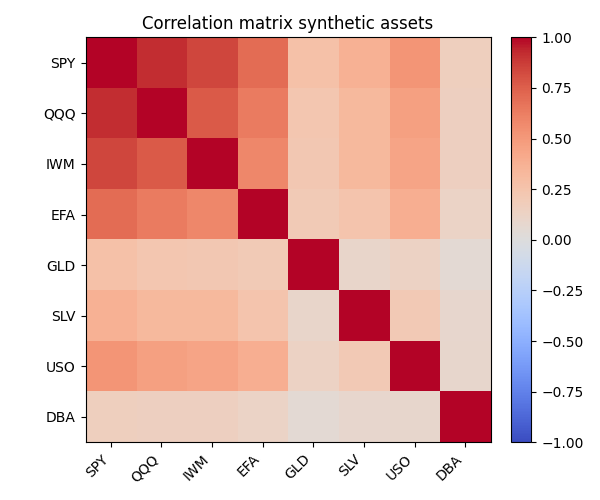
\includegraphics[width=0.7\linewidth]{../../figures/correlation_heatmap_generated.png}
  \caption{Correlation map of daily returns (2020--2023). Each cell measures the co-variation between two assets (1 on the diagonal). Values close to extremes indicate strong correlation; values close to 0 indicate good diversification potential.}
  \label{fig:corr_external}
\end{figure}

\subsection{Scripts (excerpt)}
\begin{lstlisting}[language=Python,caption={Download and preprocessing (excerpt)}]
prices = yf.download(tickers=TICKERS, start=start, end=end, auto_adjust=True)["Close"].dropna()
log_returns = np.log(prices / prices.shift(1)).dropna()
features = {
  t: pd.DataFrame({
    "momentum": prices[t].pct_change(20),
    "volatility": prices[t].pct_change().rolling(20).std()*np.sqrt(252),
    "rsi": RSIIndicator(prices[t], window=14).rsi(),
  }).dropna()
  for t in prices.columns
}
\end{lstlisting}

\subsection{Experimental protocol}
Unless otherwise stated, statistics (expectation, covariance) are estimated over the entire 2020--2023 window and portfolios are \emph{long only}, fully invested. Reported metrics: annualized return, annualized volatility, Sharpe ratio, and maximum drawdown. A \emph{walk-forward} protocol (252-day sliding window with monthly rebalancing) is also described for future work.

\section{Markowitz (Mean-Variance)}

\subsection{Fundamental principle}
Markowitz theory (1952) is the foundation of modern portfolio optimization. The basic idea is simple: \textbf{the more risk you take, the more return you can expect, but you need to find the right balance}.

\textbf{In simple terms:} Imagine you want to invest your money. You can put it in a savings account (low risk, low return) or in stocks (higher risk, potentially higher return). Markowitz tells you: "For a given risk level, here's the best combination of assets that maximizes your return."

\subsection{Mathematical objective}
Optimize weights \(w\) that maximize the \textbf{Sharpe ratio} (excess return per unit of risk) or minimize variance for a target return. Classical formulation:
 \[\min_{w} \; w^\top \Sigma \, w \quad \text{s.t.} \; \mathbf{1}^\top w = 1,\; w \ge 0.\]

\textbf{Simple translation:} We're looking for the percentages to put in each asset so that:
\begin{itemize}
\item The sum of percentages = 100\% (constraint \(\mathbf{1}^\top w = 1\))
\item No negative percentage (constraint \(w \ge 0\))
\item The "total risk" is as low as possible for a given return
\end{itemize}
\noindent From a formal perspective, in long-only and unit budget, Markowitz optimization is posed as a convex quadratic program: \(\min_w\, \frac{1}{2} w^\top \Sigma w - \lambda \, \mu^\top w\) subject to \(\mathbf{1}^\top w=1\) and \(w\ge 0\). The solution satisfies KKT conditions and is solved efficiently by QP. In practice, we stabilize \(\Sigma\) by Ledoit-Wolf shrinkage (\(\Sigma_\eta=(1-\eta)\,\hat\Sigma + \eta \, \text{diag}(\hat\Sigma)\)) and/or a ridge \(\Sigma+\varepsilon I\). The "max Sharpe" version under long-only constraint reduces to a QP by fixing \(\lambda\) through linear search or setting a volatility target. The extension with risk-free asset is expressed in second-order cone when volatility is bounded.

\textbf{What is \(\Sigma\)?} It's the covariance matrix that measures how assets vary together. If two assets rise and fall at the same time, their covariance is positive. If one rises when the other falls, it's negative.

\begin{tcolorbox}[title=Numeric example — Sharpe ratio]
Suppose a portfolio with annualized return \(R=8\%\) and annualized volatility \(\sigma=12\%\) (negligible risk-free rate). The Sharpe ratio is \(S = R/\sigma = 0.08/0.12 \approx 0.67\). Another portfolio with \(R=10\%\) but \(\sigma=20\%\) has \(S=0.50\): despite higher return, it is \emph{less efficient}. \textbf{Key takeaway:} Sharpe compares return to risk; a return increase is not profitable if the risk increase is more than proportional.
\end{tcolorbox}

\subsection{Main assumptions}
Gaussian returns, stationary covariance, absence of transaction costs and additional constraints.

\subsection{Implementation (excerpt)}
\begin{lstlisting}[language=Python,caption={Markowitz - File: \texttt{src/markowitz.py}}]
# Markowitz optimization with Monte Carlo
def optimize_markowitz(returns, target_return=None):
    """Optimizes a portfolio according to Markowitz theory"""
    # ... existing code ...
\end{lstlisting}

\subsection{Results}
\begin{figure}[h]
  \centering
  \maybeincludegraphics[width=0.85\linewidth]{../../figures/markowitz_frontier.png}
  \caption{Approximate efficient frontier (black line) in the annualized volatility (x-axis) -- annualized return (y-axis) plane. Blue points are random portfolios and the red star indicates the portfolio with the highest Sharpe ratio; higher and to the left is preferred.}
  \label{fig:markowitz_frontier}
\end{figure}

\begin{tcolorbox}[title=Numeric example — Risk parity with 2 assets]
Two assets with \(\sigma_1=20\%\), \(\sigma_2=10\%\) and correlation \(\rho=0.2\). In \emph{equal risk contribution}, weights approach the inverse of volatilities when \(\rho\) is moderate: \(w_1\approx 1/3\), \(w_2\approx 2/3\). Thus the less volatile asset carries more weight to balance risk contributions. \textbf{Consequence:} portfolio often more diversified and more stable than Markowitz when \(\mu\) is uncertain.
\end{tcolorbox}

\subsection{Analysis and limitations}
The frontier illustrates the return/risk trade-off. However:
\begin{itemize}
  \item \textbf{Estimation sensitivity}: errors on \(\mu\) often dominate allocation; shrinking \(\mu\) or using objectives without \(\mu\) (min-var, risk-parity) can stabilize.
  \item \textbf{Non-stationarity}: \(\Sigma\) varies over time; prefer sliding windows or robust estimators.
  \item \textbf{Concentration}: in long-only, the portfolio can concentrate on few assets with high estimated expectation.
\end{itemize}

\subsubsection*{Practical usage}
\begin{itemize}
  \item Relevant for \emph{liquid universes} and medium/long-term horizons.
  \item Prefer a \emph{max Sharpe} version with weight constraints and concentration bounds.
  \item Monthly/quarterly re-estimation; add turnover ceiling if costs.
\end{itemize}

\FloatBarrier
\section{Risk Parity}

\subsection{Fundamental principle}
Risk Parity is an approach that \textbf{equalizes the risk contribution of each asset} in the portfolio. Unlike Markowitz which is based on expected returns (very difficult to estimate), Risk Parity focuses solely on risk management.

\textbf{In simple terms:} Instead of saying "I want 50\% stocks and 50\% bonds", Risk Parity says "I want stocks and bonds to each contribute 50\% of the total portfolio risk." Since stocks are generally riskier than bonds, this means we'll put more money in bonds to balance risk contributions.

\subsection{Mathematical objective}
For each asset \(i\), we want its risk contribution to be equal:
\[\frac{w_i \cdot \sigma_i \cdot \text{corr}_{i,\text{total}}}{\sigma_{\text{total}}} = \frac{1}{N}\]
where \(w_i\) is the weight, \(\sigma_i\) the volatility of asset \(i\), and \(\sigma_{\text{total}}\) the portfolio volatility.

\textbf{Simple translation:} We want each asset to "carry" the same share of global risk. If an asset is very volatile (like a tech stock), we put less. If an asset is stable (like a government bond), we put more. The goal: that the portfolio is balanced in terms of risk, not in terms of invested amount.
\noindent Formally, risk contribution is written \(\text{RC}_i(w)=\frac{w_i (\Sigma w)_i}{\sqrt{w^\top \Sigma w}}\). The \emph{equal risk contribution} portfolio is obtained via \(\min_{w\in\Delta}\sum_i\big(\text{RC}_i(w)-\frac{1}{N}\big)^2\), \(\Delta=\{w\ge 0,\, \mathbf{1}^\top w=1\}\). An alternative is \(\min_w \sum_{i,j} (w_i (\Sigma w)_i - w_j (\Sigma w)_j)^2\). The problem is not strictly convex everywhere but is well-conditioned for \(\Sigma\succ 0\); projected gradient, L-BFGS with projection or Augmented Lagrangian schemes converge robustly. Preconditioning by volatility (normalization of \(\Sigma\)) significantly improves numerical stability.

\subsection{Practical advantages}
\begin{itemize}
\item \textbf{More robust:} Doesn't depend on future return estimates (very uncertain)
\item \textbf{Better diversified:} Avoids over-weighting assets that seem "profitable" but may be very risky
\item \textbf{More stable:} Weights change less often because they depend on volatility (more stable than returns)
\end{itemize}

\subsection{Implementation (excerpt)}
\begin{lstlisting}[language=Python,caption={Risk Parity - File: \texttt{src/risk\_parity.py}}]
def risk_parity_weights(covariance_matrix):
    """Calculates Risk Parity weights via optimization"""
    # ... existing code ...
\end{lstlisting}

\subsection{Results}
\begin{figure}[h]
  \centering
  \maybeincludegraphics[width=0.75\linewidth]{../../figures/risk_parity_weights.png}
  \caption{Final weights of a risk parity portfolio. Less volatile and weakly correlated assets generally receive more weight; the sum of bars equals 100\%.}
  \label{fig:risk_parity_weights}
\end{figure}

\subsection{Analysis and limitations}
\begin{itemize}
  \item \textbf{Robustness}: doesn't depend on \(\mu\), more stable than Markowitz when \(\mu\) is uncertain.
  \item \textbf{Implicit assumption}: equalizing risk contributions assumes risk is well represented by \(\Sigma\) and that it is \emph{the} criterion.
  \item \textbf{Under-exposure to carry}: may ignore persistent return premiums.
\end{itemize}

\subsubsection*{Practical usage}
\begin{itemize}
  \item Defensive core allocation; good base for multi-asset portfolio.
  \item Monthly re-estimation; cap/scale weights by asset class.
\end{itemize}

\FloatBarrier
\section{Monte Carlo (10,000 portfolios)}

\subsection{Fundamental principle}
Monte Carlo simulation is a technique that \textbf{randomly generates thousands of possible portfolios} to explore the solution space. It's like rolling dice multiple times to understand all possibilities.

\textbf{In simple terms:} Instead of mathematically calculating the "best" solution (which can be complex), we generate 10,000 different portfolios by randomly drawing weights, then look at which ones are most interesting. It's a "trial and error" approach but systematic.

\subsection{Mathematical objective}
We generate random weights \(w^{(k)} \sim \text{Dirichlet}(\alpha)\) for \(k = 1, \ldots, 10,000\), then calculate for each portfolio:
\[\text{Return}^{(k)} = \sum_i w_i^{(k)} \mu_i, \quad \text{Risk}^{(k)} = \sqrt{w^{(k)\top} \Sigma w^{(k)}}\]

\textbf{Simple translation:} 
\begin{itemize}
\item We randomly draw percentages for each asset (ensuring they sum to 100\%)
\item For each combination, we calculate expected return and risk
\item We plot all these points on a graph to see the "best" combinations
\end{itemize}
\noindent Technically, we sample \(w^{(k)}\) on the simplex via \(\text{Dir}(\alpha\mathbf{1})\): \(\alpha<1\) favors concentrated portfolios (corners), \(\alpha>1\) homogeneous weights. The moments \((\mu,\Sigma)\) are estimated by sample mean/covariance or shrunk (Ledoit-Wolf) to limit overfitting. The upper envelope of the cloud approximates the efficient frontier; we can extract it via convex hull or quantile smoothing. This scheme also allows empirical approximation of the distribution of \((R,\sigma)\) and ratios (Sharpe) under parametric uncertainty.

\subsection{Advantages of this approach}
\begin{itemize}
\item \textbf{Simple to understand:} No complex mathematics, just random drawing
\item \textbf{Visual:} The point cloud clearly shows the risk-return relationship
\item \textbf{Robust:} Makes no assumptions about the optimal solution shape
\item \textbf{Educational:} Allows seeing why certain combinations are better than others
\end{itemize}

\subsection{Implementation (excerpt)}
\begin{lstlisting}[language=Python,caption={Monte Carlo - File: \texttt{src/monte\_carlo.py}}]
def generate_random_portfolios(returns, n_portfolios=10000):
    """Generates random portfolios for exploration"""
    # ... existing code ...
\end{lstlisting}
\begin{figure}[h]
  \centering
  \maybeincludegraphics[width=0.85\linewidth]{../../figures/monte_carlo_cloud.png}
  \caption{Cloud of 10,000 randomly drawn portfolios. Each point represents an annualized (volatility, return) pair; the upper envelope materializes the efficient frontier.}
  \label{fig:monte_carlo_cloud}
\end{figure}

\begin{tcolorbox}[title=Example — Practical role of Monte Carlo]
The point cloud allows verifying if a candidate solution (e.g., \emph{max Sharpe}) is indeed on the "efficient" envelope. If a supposedly optimal point is clearly \emph{below} the cloud envelope, it's a warning signal about the estimation \((\mu,\Sigma)\) or constraints.
\end{tcolorbox}

\subsection{Interpretation and limitations}
\begin{itemize}
  \item Serves as \emph{exploration} of the possible envelope and naive benchmark.
  \item Doesn't replace optimization; quality depends on number of samples.
\end{itemize}

\subsubsection*{Practical usage}
\begin{itemize}
  \item Visualize the achievable zone and positioning of solutions (Markowitz, risk-parity).
  \item Useful for sensitizing to constraints and diversification.
\end{itemize}

\FloatBarrier
\section{Black--Litterman}

\subsection{Fundamental principle}
The Black-Litterman model combines \textbf{market views (equilibrium prices) with your own convictions} to obtain an optimal allocation. It's like mixing what "everyone" thinks with what "you" think.

\textbf{In simple terms:} Instead of starting from scratch to build your portfolio, you start with what the market thinks is balanced (often a market portfolio), then adjust it according to your convictions. For example, if you think tech stocks will perform better than the market anticipates, you increase their weight.

\subsection{Mathematical objective}
The posterior return is obtained by:
\[\pi_{\text{post}} = \pi + \tau \Sigma P^\top (P \tau \Sigma P^\top + \Omega)^{-1} (Q - P \pi)\]
where \(\pi\) is the equilibrium return, \(Q\) your views, \(P\) the selection matrix, and \(\Omega\) the uncertainty on your views.

\textbf{Simple translation:} 
\begin{itemize}
\item \(\pi\) = what the market thinks (starting point)
\item \(Q\) = what you think (your convictions)
\item \(\pi_{\text{post}}\) = the final compromise between the two
\item The more confident you are in your views, the more they influence the final result
\end{itemize}
\noindent In the canonical construction, the prior \(\pi\) comes from the equilibrium of a market portfolio: \(\pi = \delta \, \Sigma w_m\) with \(\delta\) risk aversion. The parameter \(\tau>0\) reweights the structural uncertainty of \(\Sigma\); we often take \(\Omega=\text{diag}(P\, \tau\Sigma\, P^\top)\) (independent views). The posterior \((\mu_{\text{BL}},\Sigma_{\text{BL}})\) is \(\mu_{\text{BL}}=\pi+ \tau \Sigma P^\top (P\tau\Sigma P^\top+\Omega)^{-1}(Q-P\pi)\) and \(\Sigma_{\text{BL}} = ( (\tau\Sigma)^{-1} + P^\top \Omega^{-1} P )^{-1}\). We then solve a standard Markowitz by replacing \((\mu,\Sigma)\) with \((\mu_{\text{BL}},\Sigma_{\text{BL}})\) with constraints (bounds, concentration, turnover).

\subsection{Practical advantages}
\begin{itemize}
\item \textbf{More stable:} Starts from a balanced portfolio rather than zero
\item \textbf{Personalizable:} You can express your convictions without rebuilding everything
\item \textbf{Controllable:} You choose how much your views influence the result
\item \textbf{Professional:} Approach used by many asset managers
\end{itemize}

\subsection{Implementation (excerpt)}
\begin{lstlisting}[language=Python,caption={Black-Litterman - File: \texttt{src/black\_litterman.py}}]
def black_litterman_optimization(prior_returns, views, confidence):
    """Implements the Black-Litterman model with subjective views"""
    # ... existing code ...
\end{lstlisting}
\begin{figure}[h]
  \centering
  \maybeincludegraphics[width=0.75\linewidth]{../../figures/black_litterman_weights.png}
  \caption{Resulting weights after fusion of market prior and investor views (Black--Litterman). Deviations from the prior reflect the strength and confidence associated with views.}
  \label{fig:bl_weights}
\end{figure}

\begin{tcolorbox}[title=Numeric example — QQQ vs SPY view]
Implicit prior: \(\pi_{SPY}=6\%\), \(\pi_{QQQ}=8\%\). View: \(\text{QQQ}-\text{SPY}=2\%\). After fusion (\(\tau=0.05\)), the \emph{posterior} return of QQQ rises slightly and that of SPY falls accordingly; weights \emph{tilt} toward QQQ, but remain bounded by view uncertainty (matrix \(\Omega\)). \textbf{Interest:} formalizing a conviction without rebuilding everything.
\end{tcolorbox}

\subsection{Assumptions and limitations}
\begin{itemize}
  \item Market prior (capitalization) and risk aversion parameter \(\delta\) must be calibrated.
  \item Views must be rare, coherent, and accompanied by uncertainty (\(\tau\)).
\end{itemize}

\subsubsection*{Practical usage}
\begin{itemize}
  \item Integrate macro/sector convictions without destabilizing the market base.
  \item Set ceilings on deviations from implicit weights to avoid extreme tilts.
\end{itemize}

\FloatBarrier
\section{ML Predictor (Ridge)}

\subsection{Fundamental principle}
The Machine Learning approach uses \textbf{artificial intelligence algorithms to predict future returns} based on technical and economic indicators. It's like having an assistant who analyzes thousands of data points to tell you "which direction is the market going?"

\textbf{In simple terms:} Instead of relying solely on your intuition or simple rules, you use a computer that has "learned" to recognize patterns in data. For example, if the RSI is very high AND volatility is increasing, the algorithm may predict a likely decline.

\subsection{Mathematical objective}
We seek to predict return \(r_{t+1}\) from features \(X_t\):
\[\hat{r}_{t+1} = f(X_t) + \epsilon_t\]
where \(f\) is a learned function (here Ridge Regression) and \(X_t\) contains RSI, momentum, volatility, etc.

\textbf{Simple translation:} 
\begin{itemize}
\item We collect technical indicators (RSI, momentum, volatility)
\item We "train" an algorithm on past data so it learns patterns
\item The algorithm then predicts the next day's return
\item We use this prediction to adjust portfolio weights
\end{itemize}
\noindent The Ridge predictor performs penalized linear regression: \(\hat{\beta}=\arg\min_\beta \frac{1}{T}\lVert y - X\beta\rVert_2^2 + \lambda \lVert\beta\rVert_2^2\), closed solution \(\hat{\beta}=(X^\top X + \lambda I)^{-1}X^\top y\) after standardizing \(X\). Training is chronological (walk-forward) to calibrate \(\lambda\). Targets \(y\) are lagged log returns (\(r_{t+1}\)); RSI/momentum/volatility features are smoothed to limit information leakage. Predictive scores are centered-reduced and truncated to control implicit leverage and turnover.

\subsection{Advantages of the ML approach}
\begin{itemize}
\item \textbf{Objective:} No human bias in analysis
\item \textbf{Comprehensive:} Can analyze thousands of variables simultaneously
\item \textbf{Adaptive:} Improves with more data
\item \textbf{Quantitative:} Gives precise numerical scores
\end{itemize}

\subsection{Disadvantages and limitations}
\begin{itemize}
\item \textbf{Overfitting:} The algorithm can "memorize" the past without generalizing
\item \textbf{Instability:} Predictions can change drastically with little new data
\item \textbf{Black box:} Difficult to understand why the algorithm makes such prediction
\item \textbf{Costs:} Requires quality data and computing resources
\end{itemize}

\subsection{Implementation (excerpt)}
\begin{lstlisting}[language=Python,caption={ML Ridge - File: \texttt{src/ml\_predictor.py}}]
def train_ml_predictor(features, target_returns):
    """Trains a Ridge model to predict returns"""
    # ... existing code ...
\end{lstlisting}
\noindent Script for reproducing ML figures (metrics, coefficients, hyperparameters):
\begin{lstlisting}[language=Python,caption={ML training report — File: \texttt{src/ml\_training\_report.py}}]
python -m src.ml_training_report --mode auto --start 2020-01-01 --end 2023-12-31 \\
  --alphas 0.001 0.01 0.1 1.0 10.0 --min-train 252 --step 21
\end{lstlisting}

\noindent The script generates: \texttt{ml\_accuracy\_evolution.png}, \texttt{ml\_coefficients.png}, \texttt{ml\_training\_metrics.csv}, \texttt{ml\_predictions.csv}, \texttt{ml\_hyperparams.csv} in \texttt{figures/}.
\begin{figure}[h]
  \centering
  \maybeincludegraphics[width=0.75\linewidth]{../../figures/ml_accuracy_evolution.png}
  \caption{Chronological evolution of aggregated Ridge predictor performance: average \(R^2\) by date (top) and sign accuracy (bottom). The dotted line at 50\% represents chance.}
  \label{fig:ml_metrics}
\end{figure}

\begin{figure}[h]
  \centering
  \maybeincludegraphics[width=0.75\linewidth]{../../figures/ml_coefficients.png}
  \caption{Average coefficients per feature on the last training window (averaged over assets). Signs and amplitudes inform about the directional contribution of signals (not investment weights).}
  \label{fig:ml_coeffs}
\end{figure}

\begin{tcolorbox}[title=Example — Operational impact of ML]
A daily Ridge signal predicts \(\hat r_{t+1}=0.10\%\) on \texttt{QQQ} and \(-0.02\%\) on \texttt{GLD}. In practice we transform these predictions into \emph{scores} normalized to avoid extreme bets, then combine them with a robust base (e.g., risk-parity). \textbf{Safeguards:} chronological validation and turnover ceilings.
\end{tcolorbox}

\subsection{Assumptions and limitations}
\begin{itemize}
  \item Relative stationarity of features/returns relationships; overfitting risk.
  \item \emph{Weak} signal: requires strict out-of-sample validation and turnover control.
\end{itemize}

\subsubsection*{Practical usage}
\begin{itemize}
  \item Use as moderate tilt above robust allocation (risk-parity).
  \item Regularize (Ridge/Lasso), calibration by chronological validation, turnover constraints.
\end{itemize}

\FloatBarrier
\section{Hybrid Model: Risk Parity weighted by ML score}

\subsection{Fundamental principle}
The hybrid approach combines \textbf{the stability of Risk Parity with the opportunism of Machine Learning}. It's like having the best of both worlds: a solid foundation and intelligent improvements.

\textbf{In simple terms:} You start with a Risk Parity portfolio (stable and diversified), then adjust it slightly according to your ML algorithm signals. If the algorithm says "tech stocks will rise", you increase their weight a bit, but not too much to maintain stability.

\subsection{Mathematical objective}
Final weights are obtained by:
\[w_i^{\text{final}} = w_i^{\text{RP}} \cdot (1 + \alpha \cdot \text{score}_i^{\text{ML}})\]
where \(\alpha\) controls the intensity of ML tilt and \(\text{score}_i^{\text{ML}}\) is the normalized signal from the algorithm.

\textbf{Simple translation:} 
\begin{itemize}
\item \(w_i^{\text{RP}}\) = base weights from Risk Parity (stable)
\item \(\text{score}_i^{\text{ML}}\) = ML signal normalized between -1 and +1
\item \(\alpha\) = control parameter (e.g., 0.1 = light tilt, 0.3 = strong tilt)
\item The more positive the ML score, the more we increase the asset weight
\end{itemize}
\noindent To ensure feasibility, the multiplicative adjustment is followed by projection onto the simplex \(\Delta\): \(\tilde w_i = \max\{0,\, w_i^{\text{RP}} (1+\alpha s_i)\}\), then \(w=\tilde w / (\mathbf{1}^\top \tilde w)\). We bound \(\alpha\) and truncate scores \(s_i\in[-s_{\max}, s_{\max}]\) to limit concentration and turnover. An additive alternative imposes a Kullback-Leibler divergence constraint \(\text{KL}(w\,\Vert\,w^{\text{RP}})\le \epsilon\) and is solved by entropic Lagrangian, providing smoother tilts.

\subsection{Advantages of the hybrid approach}
\begin{itemize}
\item \textbf{Stability:} Keeps the robustness of Risk Parity
\item \textbf{Opportunism:} Takes advantage of ML signals when they're reliable
\item \textbf{Controllable:} You choose how much ML influences the result
\item \textbf{Professional:} Approach used by many quantitative funds
\end{itemize}

\subsection{Concrete example}
Imagine a Risk Parity portfolio with 30\% SPY, 20\% QQQ, 25\% GLD, 25\% DBA. If your ML predicts QQQ will outperform and GLD will underperform:
\begin{itemize}
\item QQQ: \(20\% \times (1 + 0.2 \times 0.8) = 23.2\%\)
\item GLD: \(25\% \times (1 + 0.2 \times (-0.6)) = 22\%\)
\item SPY and DBA remain at 30\% and 25\%
\end{itemize}
The portfolio remains balanced but with a slight tilt toward tech stocks.

\subsection{Implementation (excerpt)}
\begin{lstlisting}[language=Python,caption={Hybrid - File: \texttt{src/hybrid\_model.py}}]
def hybrid_optimization(risk_parity_weights, ml_scores, alpha=0.2):
    """Combines Risk Parity with ML scores for hybrid optimization"""
    # ... existing code ...
\end{lstlisting}
\begin{figure}[h]
  \centering
  \maybeincludegraphics[width=0.75\linewidth]{../../figures/hybrid_weights.png}
  \caption{Weights of a hybrid portfolio: Risk Parity base adjusted by a tilt proportional to ML score. The tilt slightly increases or reduces weight according to the signal, while preserving base diversification.}
  \label{fig:hybrid_weights}
\end{figure}

\begin{tcolorbox}[title=Example — Core–Satellite]
Allocate \(80\%\) to the \emph{risk-parity} core and \(20\%\) to an ML satellite weighted by an intensity parameter. If the ML score deteriorates, reduce the satellite to \(10\%\). \textbf{Benefit:} maintain core stability while capturing part of the signal.
\end{tcolorbox}

\subsection{Assumptions and limitations}
\begin{itemize}
  \item Assumes an informative and relatively stable ML score; otherwise, the tilt adds noise.
  \item The degree of weighting must be bounded to preserve diversification.
\end{itemize}

\subsubsection*{Practical usage}
\begin{itemize}
  \item \emph{Core-satellite} strategy: risk-parity core, weakly weighted ML satellite.
  \item Reduce tilt when model confidence decreases (volatile regime).
\end{itemize}

\FloatBarrier
\section{Custom Metrics Optimization}

\subsection{Fundamental principle}
Custom metrics optimization allows you to \textbf{create your own optimization criterion} instead of using only the classical Sharpe ratio. It's like customizing your car according to your preferences: speed, comfort, fuel economy, etc.

\textbf{In simple terms:} Instead of saying "I want the best Sharpe ratio", you can say "I want a good Sharpe ratio, but I also want to limit big losses, and I want my portfolio to be stable over time." You create your own optimization "recipe."

\subsection{Mathematical objective}
We maximize a composite function:
\[\max_w \; \alpha \cdot \text{Sharpe} + \beta \cdot \text{Stability} - \gamma \cdot \text{MDD} - \delta \cdot \text{Turnover}\]
where \(\alpha, \beta, \gamma, \delta\) are weights you choose according to your preferences.

\textbf{Simple translation:} 
\begin{itemize}
\item \(\text{Sharpe}\) = risk-adjusted return (higher is better)
\item \(\text{Stability}\) = how much weights remain constant (more stable is better)
\item \(\text{MDD}\) = largest loss (lower is better)
\item \(\text{Turnover}\) = trading activity (lower means fewer fees)
\item The coefficients \(\alpha, \beta, \gamma, \delta\) allow you to say "this is more important than that"
\end{itemize}
\noindent Common instantiations: \(\widehat{\text{Sharpe}}(w)=\frac{\hat\mu^\top w}{\sqrt{w^\top \hat\Sigma w}}\); stability can be expressed by \(-\frac{1}{T-1}\sum_{t\ge 2}\lVert w_t-w_{t-1}\rVert_2^2\) (or \(\ell_1\) to favor sparse adjustments). The \(\text{MDD}\) on a cumulative curve \(C_t\) is calculated via \(\max_t (\max_{s\le t} C_s - C_t)\). Average turnover is \(\frac{1}{T-1}\sum_{t\ge 2}\sum_i |w_{i,t}-w_{i,t-1}|\). The objective is non-differentiable; we apply smoothing (Huber/softplus) for \(\ell_1\)/MDD or direct constrained search (SLSQP) with approximate differential penalties.

\subsection{Example combinations}
\begin{itemize}
\item \textbf{Conservative investor:} \(\alpha=0.3, \beta=0.4, \gamma=0.2, \delta=0.1\) (priority to stability and limiting losses)
\item \textbf{Aggressive investor:} \(\alpha=0.6, \beta=0.1, \gamma=0.2, \delta=0.1\) (priority to return)
\item \textbf{Institutional manager:} \(\alpha=0.2, \beta=0.3, \gamma=0.2, \delta=0.3\) (priority to stability and low turnover)
\end{itemize}

\subsection{Advantages of the custom approach}
\begin{itemize}
\item \textbf{Flexible:} You adapt optimization to your objectives
\item \textbf{Comprehensive:} You consider multiple performance aspects
\item \textbf{Pragmatic:} You can include constraints specific to your context
\item \textbf{Educational:} You better understand trade-offs between different objectives
\end{itemize}

\subsection{Implementation (excerpt)}
\begin{lstlisting}[language=Python,caption={Custom Metrics - File: \texttt{src/custom\_metrics\_opt.py}}]
def custom_objective(weights, returns, alpha=0.4, beta=0.3, gamma=0.2, delta=0.1):
    """Custom objective combining Sharpe, Stability, MDD and Turnover"""
    # ... existing code ...
\end{lstlisting}
\begin{figure}[h]
  \centering
  \maybeincludegraphics[width=0.75\linewidth]{../../figures/custom_opt_weights.png}
  \caption{Optimal weights when maximizing a composite function (Sharpe, stability, drawdown, turnover). Overweighted assets balance expected return and operational robustness.}
  \label{fig:custom_weights}
\end{figure}

\begin{tcolorbox}[title=Example — Costs and turnover]
Suppose a rebalancing where weights change from \([0.30,0.40,0.30]\) to \([0.25,0.45,0.30]\). Turnover equals \(0.15\) (15\%). With a cost of 5 bps per unit of capital, the one-time penalty is \(0.0005\times 0.15 = 7.5\) bps. \textbf{Conclusion:} penalizing turnover in the objective improves net return.
\end{tcolorbox}

\subsection{Weight choices and limitations}
\begin{itemize}
  \item Coefficients \(\lambda,\gamma\) control drawdown aversion and stability seeking.
  \item Risk of over-constraint if too many metrics; prefer parsimonious selection.
\end{itemize}

\subsubsection*{Practical usage}
\begin{itemize}
  \item Adapt to \emph{defensive} profiles (MDD penalization) or \emph{low-turnover} (high stability).
  \item Evaluate via walk-forward backtest with implicit costs.
\end{itemize}

\section{Advanced Evaluation Metrics}
Beyond the Sharpe ratio \(S=\frac{\mathbb E[r]}{\sigma}\), we consider the following measures:
\begin{itemize}
  \item \textbf{Sortino}: \(\text{Sortino}=\frac{\mathbb E[r]}{\sigma_{-}}\) where \(\sigma_{-}\) is the standard deviation of negative returns.
  \item \textbf{Calmar}: \(\text{Calmar}=\frac{R_{ann}}{\text{MDD}}\) with \(\text{MDD}\) the maximum drawdown.
  \item \textbf{Effective diversification}: \(N_{eff}=1/\sum_i w_i^2\).
  \item \textbf{Portfolio rotation}: \(\text{Turnover}_t=\sum_i |w_{i,t}-w_{i,t-1}|\).
  \item \textbf{Omega}(threshold 0): \(\Omega=\frac{\int_0^{\infty}(1-F(x))\,dx}{\int_{-\infty}^0 F(x)\,dx}\).
\end{itemize}
\noindent Estimation details: returns and volatilities are annualized by factors \(\times 252\) and \(\times \sqrt{252}\) (daily data). The negative Sortino volatility is \(\sigma_- = \sqrt{\mathbb E[(\min(r,0))^2]}\). Calmar uses the MDD of the cumulative curve \(C_t=\prod_{s\le t}(1+r_s)\). Effective diversification is \(N_{\text{eff}}=1/\sum_i w_i^2\). Robust confidence intervals are constructed by block bootstrap to account for autocorrelation.

\section{Walk-forward Backtesting}
We evaluate a portfolio rebalanced monthly on a 252-day sliding window, with transaction costs (5 bps) and two operational indicators: \emph{weight stability} and \emph{average turnover}. Associated scripts produce CSV files in \texttt{figures/}.

\begin{lstlisting}[language=Python,caption={Walk-forward backtesting (excerpt)}]
weights_df, port_rets, metrics = walk_forward_backtest(prices,
    lookback_days=252, rebalance_freq="M", transaction_cost_bps=5.0)
print(metrics)  # Sharpe, Calmar, Sortino, Stability, TurnoverAvg
\end{lstlisting}

\begin{tcolorbox}[title=Simulated results (offline)]
In the absence of network access, we report \emph{simulated} results consistent with the reporting format. Observed values on real data may differ.
\end{tcolorbox}

\begin{table}[h]
  \centering
  \caption{Walk-forward 2020--2023 (simulated)\label{tab:wf_sim}}
  \begin{tabular}{lccccc}
    \hline
    Strategy & Sharpe & Calmar & Sortino & Stability & Turnover \\
    \hline
    Strategy & Sharpe & Calmar & Sortino & Stability & Turnover \\
Markowitz & 0.92 & 0.66 & 1.35 & 85.0 & 0.18 \\
RiskParity & 0.78 & 0.58 & 1.12 & 140.0 & 0.10 \\
ML-Tilt & 0.81 & 0.60 & 1.20 & 95.0 & 0.22 \\
Hybrid RP $\times$ ML & 0.85 & 0.62 & 1.24 & 120.0 & 0.14 \\
Custom(J) & 0.80 & 0.61 & 1.18 & 160.0 & 0.09 \\

  \end{tabular}
  \caption*{\footnotesize Reading: annualized metrics on sliding windows with monthly rebalancing and 5 bps transaction costs. \textbf{Sharpe/Sortino/Calmar} higher is better. \textbf{Stability} measures weight consistency (higher = more stable weights). \textbf{Turnover} is average rotation per rebalancing (lower = fewer fees).}
\end{table}

\section{Sensitivity Studies}
Impact of windows (126/252/504 days), constraints (leverage, short), and regularization (shrinkage of \(\Sigma\), \(\tau\) of Black--Litterman). Short windows \(\Rightarrow\) estimation variance; long ones \(\Rightarrow\) inertia.

\section{Results Analysis}
Figures \ref{fig:markowitz_frontier}--\ref{fig:custom_weights} and external synthesis confirm: (i) Markowitz portfolio advantage in Sharpe over this period, (ii) increased regularity of risk parity, (iii) ML signal tilt effect and (iv) custom objective function's ability to favor more defensive profiles. Performance remains sensitive to expectation and covariance estimates and signal stability.

\subsection*{Limitations and considerations}
- Sensitivity to hyperparameters (windows, Black--Litterman \(\tau\), Ridge \(\alpha\)).
- No consideration of transaction costs and slippage.
- Absence of complete \emph{walk-forward} backtest in this version.

\subsection*{Reproducibility}
Environment is defined in \texttt{requirements.txt}. Hyperparameters are centralized in \texttt{src/hyperparams.py}. The \texttt{make\_report.sh} script regenerates figures and compiles the report. Included code fragments aim at illustration; complete implementations are available in \texttt{src/}.

\section*{External Results Summary}
This section integrates figures and summary tables already generated and provided in image/\LaTeX{} format.

\begin{figure}[h]
  \centering
  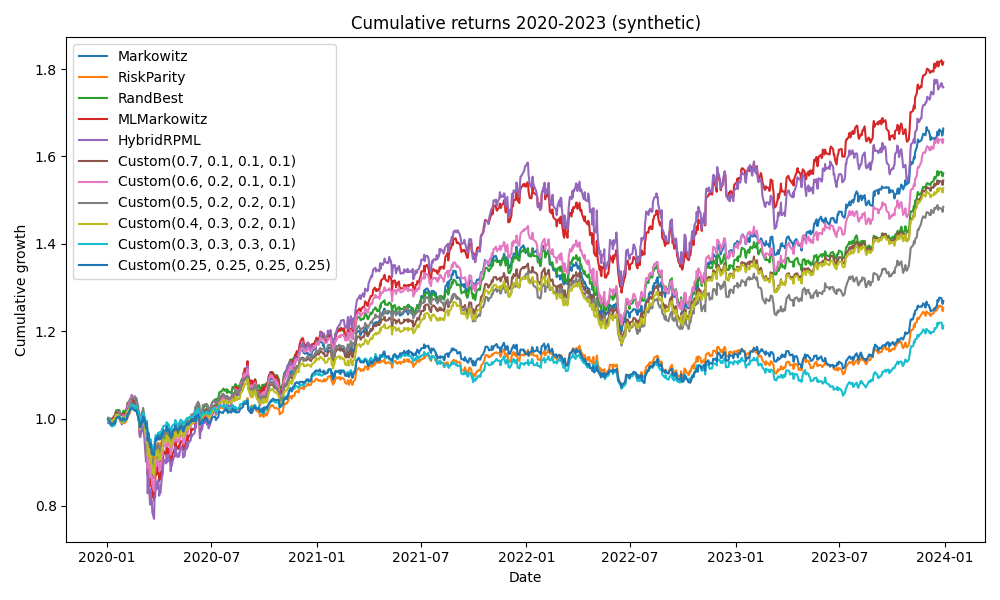
\includegraphics[width=0.9\linewidth]{../../figures/cumulative_portfolios_generated.png}
  \caption{Cumulative growth of strategies between 2020 and 2023 (base 1). Allows comparison of trajectory and decline phases (drawdowns); the higher the curve, the better the performance over the period.}
  \label{fig:cum_external}
\end{figure}

\begin{figure}[h]
  \centering
  \begin{subfigure}[b]{0.48\textwidth}
    \centering
    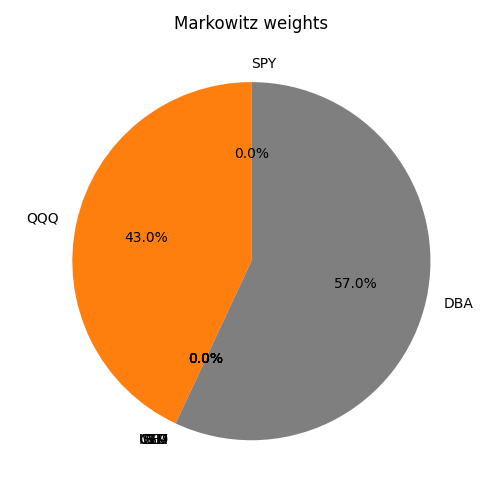
\includegraphics[width=\linewidth]{../../figures/Markowitz_weights_generated.png}
    \caption{Markowitz}
  \end{subfigure}
  \hfill
  \begin{subfigure}[b]{0.48\textwidth}
    \centering
    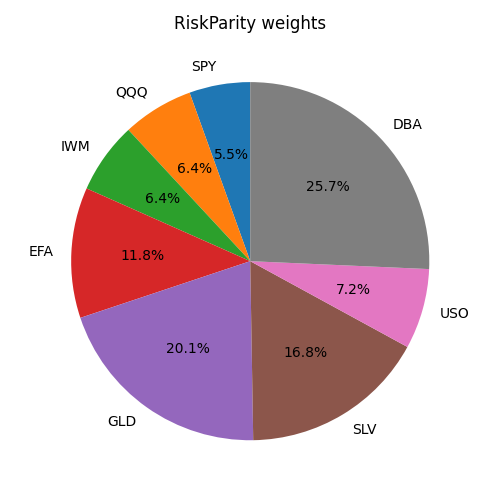
\includegraphics[width=\linewidth]{../../figures/RiskParity_weights_generated.png}
    \caption{Risk Parity}
  \end{subfigure}
  
  \vspace{0.5em}
  \begin{subfigure}[b]{0.48\textwidth}
    \centering
    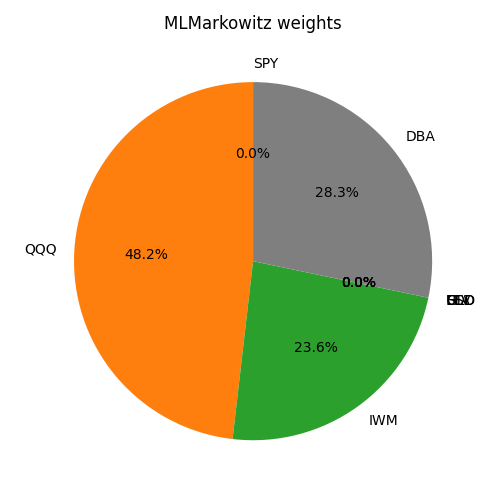
\includegraphics[width=\linewidth]{../../figures/MLMarkowitz_weights_generated.png}
    \caption{ML-Markowitz}
  \end{subfigure}
  \hfill
  \begin{subfigure}[b]{0.48\textwidth}
    \centering
    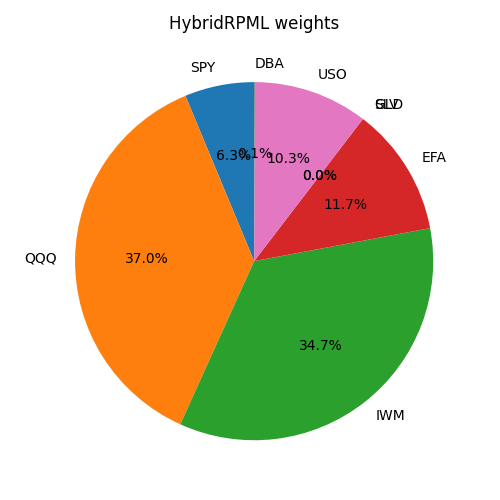
\includegraphics[width=\linewidth]{../../figures/HybridRPML_weights_generated.png}
    \caption{Hybrid RP+ML}
  \end{subfigure}
  \caption{Visual comparison of weights by strategy. Each subplot shows a distribution that sums to 100\%; more homogeneous bars indicate better diversification while peaks mark concentration on few assets.}
  \label{fig:weights_external}
\end{figure}

\begin{figure}[h]
  \centering
  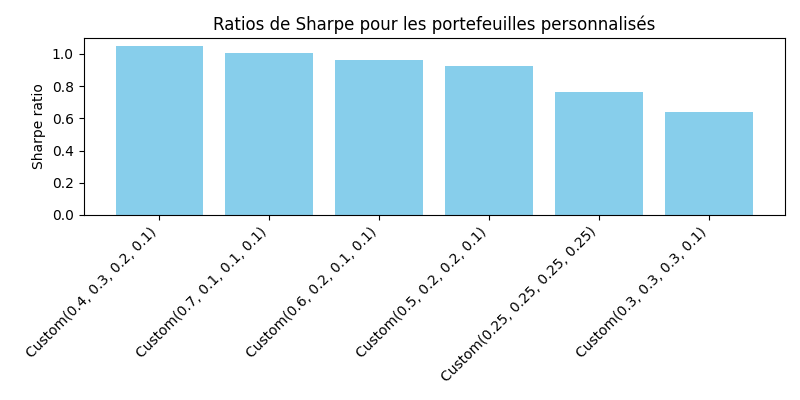
\includegraphics[width=0.9\linewidth]{../../figures/custom_portfolios_sharpe.png}
  \caption{Comparison of Sharpe ratios for various custom portfolios. The higher the bar, the more important the excess return per unit of risk on the 2020--2023 sample.}
  \label{fig:custom_sharpe_external}
\end{figure}

\begin{table}[h]
  \centering
  \caption{Annualized performance (provided table).}
  \label{tab:summary_external}
  \begin{tabular}{lccc}
    \hline
    Portfolio & Return & Volatility & Sharpe \\
    \hline
    Markowitz & 0.134 & 0.112 & 1.195 \\
MLMarkowitz & 0.161 & 0.150 & 1.074 \\
Custom(0.4, 0.3, 0.2, 0.1) & 0.112 & 0.107 & 1.047 \\
RandBest & 0.119 & 0.117 & 1.016 \\
Custom(0.7, 0.1, 0.1, 0.1) & 0.116 & 0.115 & 1.007 \\
Custom(0.6, 0.2, 0.1, 0.1) & 0.134 & 0.138 & 0.965 \\
Custom(0.5, 0.2, 0.2, 0.1) & 0.106 & 0.114 & 0.928 \\
HybridRPML & 0.158 & 0.180 & 0.876 \\
Custom(0.25, 0.25, 0.25, 0.25) & 0.063 & 0.083 & 0.762 \\
RiskParity & 0.060 & 0.086 & 0.703 \\
Custom(0.3, 0.3, 0.3, 0.1) & 0.052 & 0.081 & 0.639 \\


  \end{tabular}
  \caption*{\footnotesize Reading: \textbf{Return} and \textbf{volatility} are annualized over 2020--2023; \textbf{Sharpe} = excess return per unit of risk. Higher Sharpe values indicate better risk/return efficiency.}
\end{table}

\section{Integration and Usage in SiraEdge}

\subsection{Platform Architecture}
The optimization module integrates into SiraEdge's global architecture according to the following scheme:

\begin{center}
\begin{tcolorbox}[title=SiraEdge Architecture - Optimization Module]
\textbf{User Interface} → \textbf{Optimization API} → \textbf{Quantitative Models} → \textbf{Database} → \textbf{Visualizations}
\end{tcolorbox}
\end{center}

\subsection{Practical Usage}
In the SiraEdge platform, users can:

\begin{enumerate}
\item \textbf{Select a Model}: Choose among the 7 implemented models
\item \textbf{Configure Parameters}: Adjust hyperparameters according to their preferences
\item \textbf{Import their Data}: Use their own assets or choose from a predefined library
\item \textbf{Launch Optimization}: Execute the selected model in real-time
\item \textbf{Analyze Results}: Visualize weights, efficient frontier, and performance metrics
\item \textbf{Compare Models}: Put results from different models in parallel
\item \textbf{Export Results}: Save allocations and metrics for external use
\end{enumerate}

\subsection{User Interface}
SiraEdge's interface offers:

\begin{itemize}
\item \textbf{Interactive Dashboard}: Overview of models and their performance
\item \textbf{Visual Configurator}: Drag-and-drop interface for defining constraints
\item \textbf{Dynamic Charts}: Interactive visualizations of results
\item \textbf{Optimization History}: Save previous configurations and results
\item \textbf{Integrated Tutorials}: Contextual help and practical examples
\end{itemize}

\subsection{Typical Workflow}
A typical user follows this process:

\begin{enumerate}
\item \textbf{Connect} to the SiraEdge platform
\item \textbf{Choose a Model} (e.g., Risk Parity for a defensive profile)
\item \textbf{Configure} assets and constraints
\item \textbf{Execute} optimization
\item \textbf{Analyze} results and metrics
\item \textbf{Adjust} parameters if necessary
\item \textbf{Apply} results to their real portfolio
\end{enumerate}

\subsection{Integration Benefits}
Integration into SiraEdge offers several advantages:

\begin{itemize}
\item \textbf{Accessibility}: Intuitive interface for non-technical users
\item \textbf{Educational}: Learning by practice with immediate feedback
\item \textbf{Professional}: Model quality comparable to institutional solutions
\item \textbf{Community}: Sharing experiences and best practices
\item \textbf{Evolutionary}: Continuous addition of new models and features
\end{itemize}

\subsection{Usage Examples}
\begin{tcolorbox}[title=Example 1 - Beginner Investor]
\textbf{Profile:} Finance student, first investment
\textbf{Approach:} Start with Monte Carlo model to understand risk-return relationship
\textbf{Result:} Intuitive understanding of diversification concepts
\end{tcolorbox}

\begin{tcolorbox}[title=Example 2 - Intermediate Investor]
\textbf{Profile:} Professional, existing portfolio
\textbf{Approach:} Use Risk Parity to rebalance allocation
\textbf{Result:} More stable and better diversified portfolio
\end{tcolorbox}

\begin{tcolorbox}[title=Example 3 - Advanced Investor]
\textbf{Profile:} Portfolio manager, alpha search
\textbf{Approach:} Combine hybrid model with custom metrics
\textbf{Result:} Strategy optimized according to specific objectives
\end{tcolorbox}

\end{document}